\documentclass{article}
\usepackage{tikz}

\begin{document} 


\begin{tikzpicture}
\coordinate (A) at (2,1);
\pgfgetlastxy{\ax}{\ay}    
\fill[red] (\ax,\ay) circle (5pt);
\end{tikzpicture} 

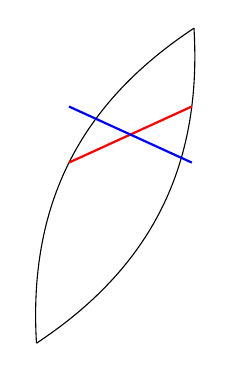
\begin{tikzpicture}
 \draw (0,0) to [bend left]  coordinate[pos=.5] (B)(2,4);
% \draw (0,0) to [bend left]  coordinate[pos=.5] (B)(2,4);\pgfgetlastxy{\bx}{\by}
 \draw (0,0) to [bend right] coordinate[pos=.8] (C)(2,4);
  \path (B);\pgfgetlastxy{\bx}{\by} 
  \path (C);\pgfgetlastxy{\cx}{\cy} 
  \draw[red,thick] (\bx,\by)--(\cx,\cy) ;
  \draw[blue,thick] (\cx,\by)--(\bx,\cy) ;
\end{tikzpicture}

\end{document} 
